% Options for packages loaded elsewhere
\PassOptionsToPackage{unicode}{hyperref}
\PassOptionsToPackage{hyphens}{url}
%
\documentclass[
]{article}
\usepackage{amsmath,amssymb}
\usepackage{lmodern}
\usepackage{ifxetex,ifluatex}
\ifnum 0\ifxetex 1\fi\ifluatex 1\fi=0 % if pdftex
  \usepackage[T1]{fontenc}
  \usepackage[utf8]{inputenc}
  \usepackage{textcomp} % provide euro and other symbols
\else % if luatex or xetex
  \usepackage{unicode-math}
  \defaultfontfeatures{Scale=MatchLowercase}
  \defaultfontfeatures[\rmfamily]{Ligatures=TeX,Scale=1}
\fi
% Use upquote if available, for straight quotes in verbatim environments
\IfFileExists{upquote.sty}{\usepackage{upquote}}{}
\IfFileExists{microtype.sty}{% use microtype if available
  \usepackage[]{microtype}
  \UseMicrotypeSet[protrusion]{basicmath} % disable protrusion for tt fonts
}{}
\makeatletter
\@ifundefined{KOMAClassName}{% if non-KOMA class
  \IfFileExists{parskip.sty}{%
    \usepackage{parskip}
  }{% else
    \setlength{\parindent}{0pt}
    \setlength{\parskip}{6pt plus 2pt minus 1pt}}
}{% if KOMA class
  \KOMAoptions{parskip=half}}
\makeatother
\usepackage{xcolor}
\IfFileExists{xurl.sty}{\usepackage{xurl}}{} % add URL line breaks if available
\IfFileExists{bookmark.sty}{\usepackage{bookmark}}{\usepackage{hyperref}}
\hypersetup{
  pdftitle={Methods},
  hidelinks,
  pdfcreator={LaTeX via pandoc}}
\urlstyle{same} % disable monospaced font for URLs
\usepackage[margin=1in]{geometry}
\usepackage{longtable,booktabs,array}
\usepackage{calc} % for calculating minipage widths
% Correct order of tables after \paragraph or \subparagraph
\usepackage{etoolbox}
\makeatletter
\patchcmd\longtable{\par}{\if@noskipsec\mbox{}\fi\par}{}{}
\makeatother
% Allow footnotes in longtable head/foot
\IfFileExists{footnotehyper.sty}{\usepackage{footnotehyper}}{\usepackage{footnote}}
\makesavenoteenv{longtable}
\usepackage{graphicx}
\makeatletter
\def\maxwidth{\ifdim\Gin@nat@width>\linewidth\linewidth\else\Gin@nat@width\fi}
\def\maxheight{\ifdim\Gin@nat@height>\textheight\textheight\else\Gin@nat@height\fi}
\makeatother
% Scale images if necessary, so that they will not overflow the page
% margins by default, and it is still possible to overwrite the defaults
% using explicit options in \includegraphics[width, height, ...]{}
\setkeys{Gin}{width=\maxwidth,height=\maxheight,keepaspectratio}
% Set default figure placement to htbp
\makeatletter
\def\fps@figure{htbp}
\makeatother
\setlength{\emergencystretch}{3em} % prevent overfull lines
\providecommand{\tightlist}{%
  \setlength{\itemsep}{0pt}\setlength{\parskip}{0pt}}
\setcounter{secnumdepth}{5}
\ifluatex
  \usepackage{selnolig}  % disable illegal ligatures
\fi
\newlength{\cslhangindent}
\setlength{\cslhangindent}{1.5em}
\newlength{\csllabelwidth}
\setlength{\csllabelwidth}{3em}
\newenvironment{CSLReferences}[2] % #1 hanging-ident, #2 entry spacing
 {% don't indent paragraphs
  \setlength{\parindent}{0pt}
  % turn on hanging indent if param 1 is 1
  \ifodd #1 \everypar{\setlength{\hangindent}{\cslhangindent}}\ignorespaces\fi
  % set entry spacing
  \ifnum #2 > 0
  \setlength{\parskip}{#2\baselineskip}
  \fi
 }%
 {}
\usepackage{calc}
\newcommand{\CSLBlock}[1]{#1\hfill\break}
\newcommand{\CSLLeftMargin}[1]{\parbox[t]{\csllabelwidth}{#1}}
\newcommand{\CSLRightInline}[1]{\parbox[t]{\linewidth - \csllabelwidth}{#1}\break}
\newcommand{\CSLIndent}[1]{\hspace{\cslhangindent}#1}

\title{Methods}
\author{}
\date{\vspace{-2.5em}}

\begin{document}
\maketitle

\hypertarget{methods}{%
\section{Methods}\label{methods}}

\hypertarget{datasets}{%
\subsection{Datasets}\label{datasets}}

\hypertarget{climate-change-scenarios}{%
\subsubsection{Climate change scenarios}\label{climate-change-scenarios}}

In order to evaluate possible scenarios of climate change in the area, we used a polygon comprising the Los Lagos and Los Ríos regions in Chile, and compared them using GCM compareR (Fajardo et al. 2020), considering Mean Annual Temperature and Annual Precipitation. The resulting scaled table of comparison among futures was then use to select models to be used in the project.

We used the simple structure index (ssi) as implemented by the Vegan package (Oksanen et al. 2019; Dolnicar et al. 1999) to test what number of clusters (Between two and eight), was the best way to represent the 32 Compared GCMs. The best representation was five clusters, from each cluster the GCM closest to the centroid of the cluster was selected. The five selected GCMS were cesm1\_bgc, gfdl\_esm2g, ipsl\_cm5a\_lr, miroc\_esm\_chem and mpi\_esm\_lr and the selected GCMs together with the clusters are shown in figure \ref{fig:SelectedGCMs}. We used the bioclimatic variables from Chelsa as predictors (Karger et al. 2017), together with the population density extracted from (Columbia University 2018).

\begin{figure}
\centering
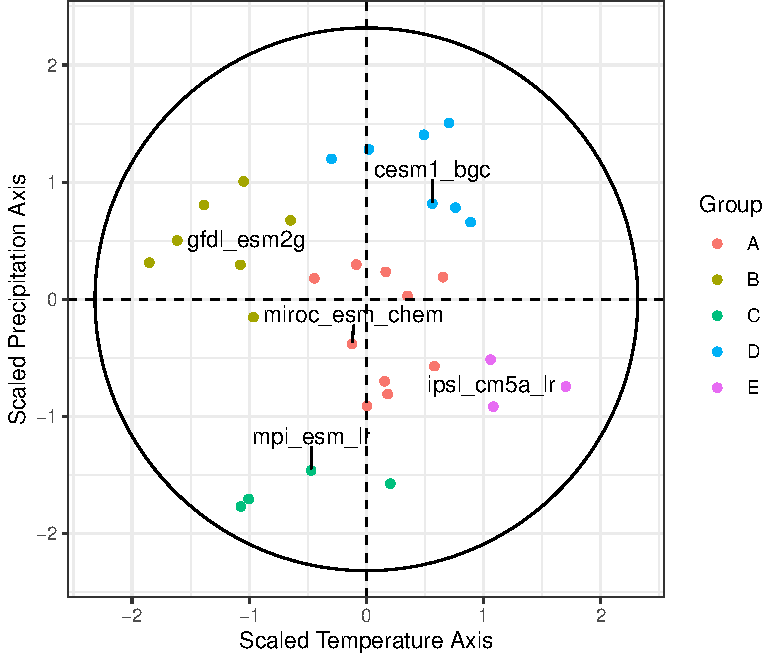
\includegraphics{Methods_files/figure-latex/SelectedGCMs-1.pdf}
\caption{\label{fig:SelectedGCMs}In this graph we can see the scaled temperature and precipitation axis, the center of the graph represent the ensemble of all models, the five groups represent the clusters selected using kmeans for five groups, the selected GCM of each cluster is shown with a label}
\end{figure}

\hypertarget{boosted-regresion-trees}{%
\subsection{Boosted Regresion Trees}\label{boosted-regresion-trees}}

We used boosted regression trees (BRTs) to fit models because they offer several advantages over other regression techniques. BRTs are a type of machine learning technique that seeks to optimize the predictive accuracy of out-of-sample data in an iterative process and using an ensemble of regression trees. By focusing on prediction, BRTs can provide a better estimate of predictive accuracy in contrast to traditional generalized linear models (e.g., linear regression). They tend to avoid including irrelevant variables, and interactions between variables are inherently included without the need to specify them a priori (Friedman 2001; Friedman and Meulman 2003). Furthermore BRTs can fit any shape of response, and hence avoid the possibility of underfitting. However, due to this flexibility, cross validation is necessary in order to avoid overfitting. Since BRTs depend on tree-based methods, the number of bifurcations of each variable together with the reduction of the residual error in each of those can be used to calculate the relative influence of each variable (Friedman and Popescu 2008; Greenwell et al. 2020).
For each training set we did a 10 fold structured cross-validation to reduce overfitting, selecting the best model optimizing the value of Root Mean Squared Error (RSME) following (Kuhn and Johnson 2013) using the caret package (Kuhn 2008) and boosted regression trees through the gbm package (Greenwell et al. 2020).

\hypertarget{generated-model}{%
\subsection{Generated model}\label{generated-model}}

We fitted a binomial Boosted Regression Trees, using a 10 fold structured cross-validation, where folds were spatially structured by using K-means were the points of each fold is shown in figure \ref{fig:kmeans}. This arrengement was made in order to diminish overfitting. Ecological data are often autocorrelated---i.e.~observations close to each other (in space or time) are more similar than distant ones (Legendre 1993). In our model this is true of the response and the predictor variables. Spatially-separated training and testing datasets can help test whether the model performs as well in nearby locations as it does in more distant places (Telford and Birks 2009). If it does not, structure might not be properly accounted for in the model or the model might be over-fitted to the training data (F. Dormann et al. 2007; Roberts et al. 2017).

\begin{figure}
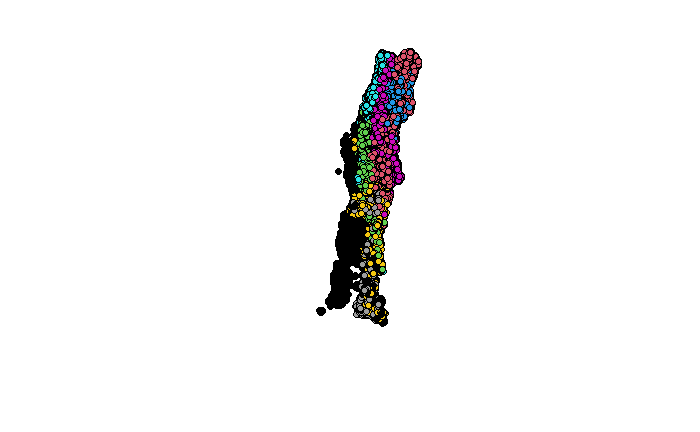
\includegraphics[width=9.72in]{Kmeans} \caption{Each point is a point used for training, each color is one of the 10 folds for the crossvalidation}\label{fig:kmeans}
\end{figure}

The accuracy of the trained model is 0.89 tested on a 20\% leftover points. The 10 most important variables oredered by relative influence are shown in figure \ref{fig:VarImp}, the top 3 variables are markedly higher than the rest, where population, the precipitation of the driest month and temperature seasonality are the most important variables, which has perfect mechanistic sense.

\begin{figure}
\centering
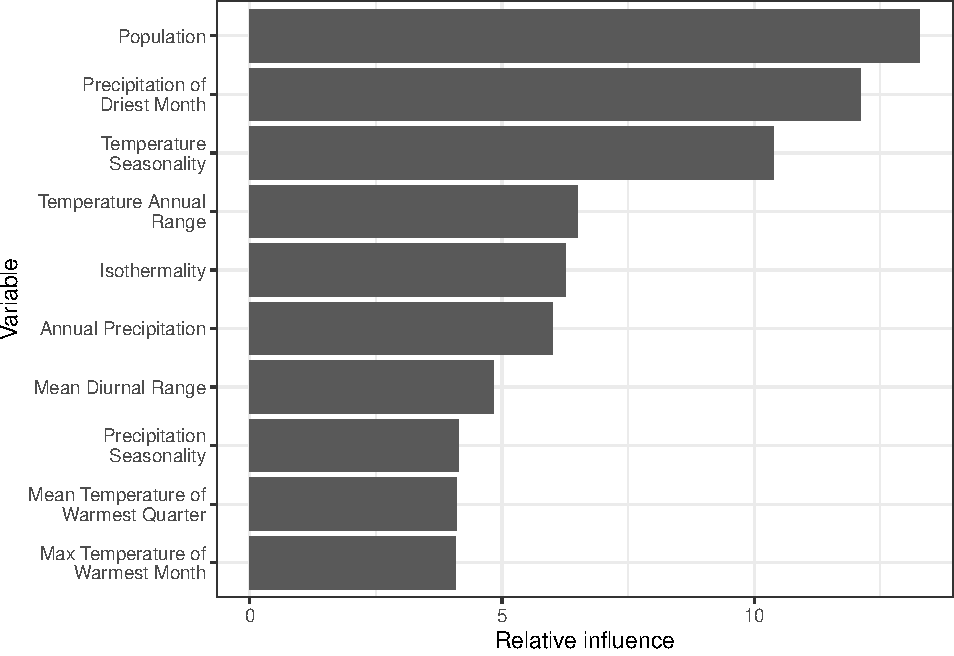
\includegraphics{Methods_files/figure-latex/VarImp-1.pdf}
\caption{\label{fig:VarImp}Top 10 variables ordered by relative influence for the Boosted Regression Tree model}
\end{figure}

\hypertarget{results}{%
\section{Results}\label{results}}

In figure \ref{fig:PredsFire} we see the predicted probability of fire predicted using the model against current conditions and 5 future GCMs for rcp 8.5, this is probably an under prediction, since we changed climate, but we don't have spatial projections on how population will change in the area, and this is the most important variable as seen in figure \ref{fig:VarImp}. This predictions are for all of the Los Lagos and Los Ríos regions, showing the study area as a white polygon.

\begin{figure}
\centering
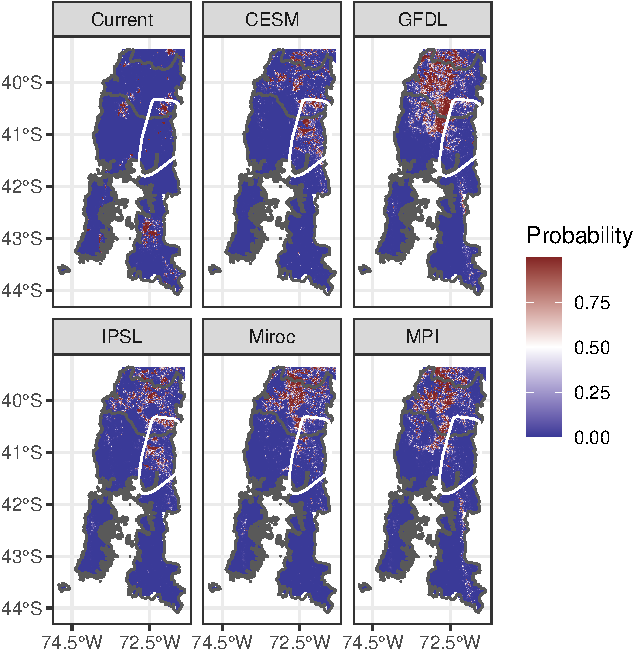
\includegraphics{Methods_files/figure-latex/PredsFire-1.pdf}
\caption{\label{fig:PredsFire}Probability of a fire happening within 20 years, for the present and for 5 differet GCMs for 2070 for the Los Lagos and Los Ríos region, in white, the area with the protected areas in the study}
\end{figure}

When we look at the predictions within the study area (figue \ref{fig:PredsFireFocus} and \ref{fig:PredsDiff}), we see that in the CESM and IPSL GCMs is there seems to be more area with an increase of fire probability, not necessarily within the protected areas, but within its vecinity as defined by the generated buffer.

\begin{figure}
\centering
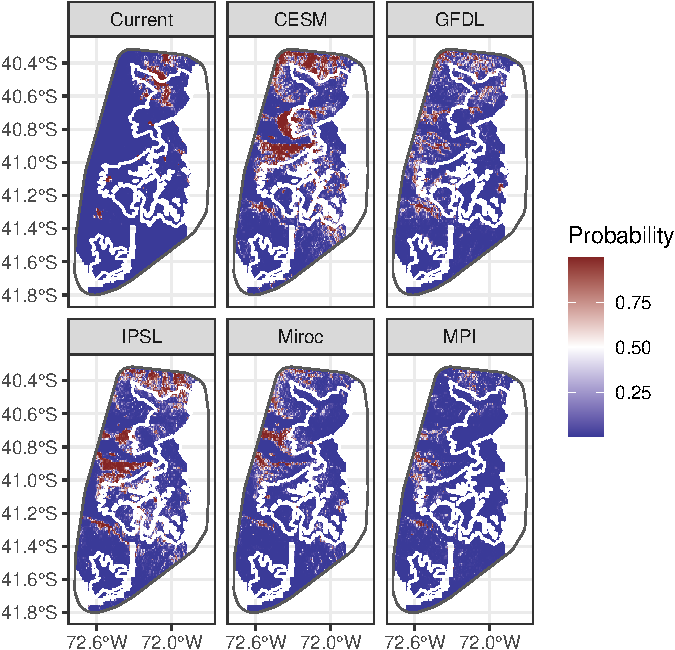
\includegraphics{Methods_files/figure-latex/PredsFireFocus-1.pdf}
\caption{\label{fig:PredsFireFocus}Probability of a fire happening within 20 years, for the present and for 5 differet GCMs for 2070 zoomed in the study area, in white, the limits of the protected areas}
\end{figure}

\begin{figure}
\centering
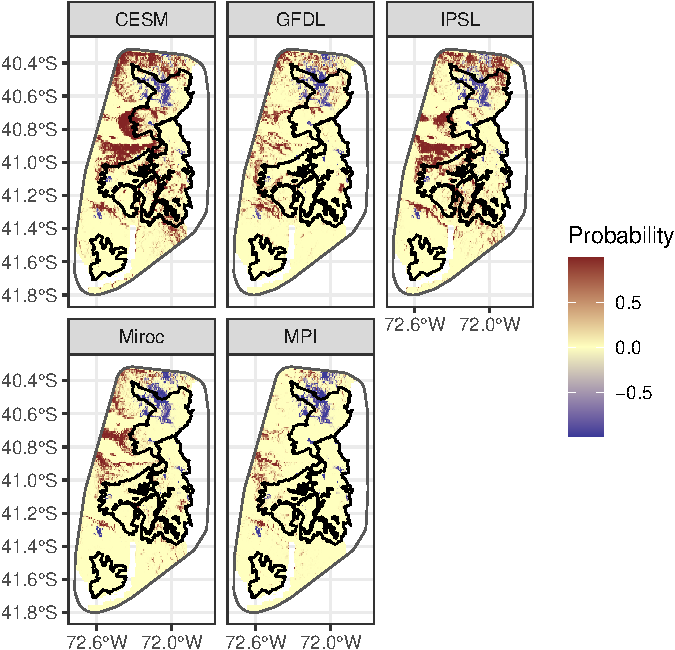
\includegraphics{Methods_files/figure-latex/PredsDiff-1.pdf}
\caption{\label{fig:PredsDiff}Difference of a fire probability (future - present), for 5 differet GCMs for 2070 zoomed in the study area}
\end{figure}

\hypertarget{references}{%
\section*{References}\label{references}}
\addcontentsline{toc}{section}{References}

\hypertarget{refs}{}
\begin{CSLReferences}{1}{0}
\leavevmode\hypertarget{ref-ColumbiaUniversity2018}{}%
Columbia University, Center for International Earth Science Information Network -. CIESIN. 2018. {``Gridded Population of the World, Version 4 (GPWv4): Population Density Adjusted to Match 2015 Revision UN WPP Country Totals, Revision 11.''} Palisades, NY: NASA Socioeconomic Data; Applications Center (SEDAC). \url{https://doi.org/10.7927/H4F47M65}.

\leavevmode\hypertarget{ref-dolnicar1999tale}{}%
Dolnicar, Sara, Klaus Grabler, Josef A Mazanec, and others. 1999. \emph{A Tale of Three Cities: Perceptual Charting for Analysing Destination Images.} CABI Publishing.

\leavevmode\hypertarget{ref-Dormann2007methods}{}%
F. Dormann, Carsten, Jana M. McPherson, Miguel B. Araújo, Roger Bivand, Janine Bolliger, Gudrun Carl, Richard G. Davies, et al. 2007. {``Methods to Account for Spatial Autocorrelation in the Analysis of Species Distributional Data: A Review.''} \emph{Ecography} 30 (5): 609--28.

\leavevmode\hypertarget{ref-fajardo2020gcm}{}%
Fajardo, Javier, Derek Corcoran, Patrick R Roehrdanz, Lee Hannah, and Pablo A Marquet. 2020. {``GCM compareR: A Web Application to Assess Differences and Assist in the Selection of General Circulation Models for Climate Change Research.''} \emph{Methods in Ecology and Evolution} 11 (5): 656--63.

\leavevmode\hypertarget{ref-Friedman2001-vj}{}%
Friedman, Jerome H. 2001. {``Greedy Function Approximation: A Gradient Boosting Machine.''} \emph{Ann. Stat.} 29 (5): 1189--1232.

\leavevmode\hypertarget{ref-Friedman2003-tl}{}%
Friedman, Jerome H, and Jacqueline J Meulman. 2003. {``Multiple Additive Regression Trees with Application in Epidemiology.''} \emph{Stat. Med.} 22 (9): 1365--81.

\leavevmode\hypertarget{ref-Friedman2008-ep}{}%
Friedman, Jerome H, and Bogdan E Popescu. 2008. {``Predictive Learning via Rule Ensembles.''} \emph{Ann. Appl. Stat.} 2 (3): 916--54.

\leavevmode\hypertarget{ref-Greenwell2020-lk}{}%
Greenwell, Brandon, Bradley Boehmke, Jay Cunningham, and G B M Developers. 2020. \emph{Gbm: Generalized Boosted Regression Models}.

\leavevmode\hypertarget{ref-karger2017climatologies}{}%
Karger, Dirk Nikolaus, Olaf Conrad, Jürgen Böhner, Tobias Kawohl, Holger Kreft, Rodrigo Wilber Soria-Auza, Niklaus E Zimmermann, H Peter Linder, and Michael Kessler. 2017. {``Climatologies at High Resolution for the Earth's Land Surface Areas.''} \emph{Scientific Data} 4 (1): 1--20.

\leavevmode\hypertarget{ref-Kuhn2008-cc}{}%
Kuhn, Max. 2008. {``Building Predictive Models in {R} Using the Caret Package.''} \emph{Journal of Statistical Software} 28 (5): 1--26.

\leavevmode\hypertarget{ref-Kuhn2013-cp}{}%
Kuhn, Max, and Kjell Johnson. 2013. \emph{Applied Predictive Modeling}. Vol. 26. Springer.

\leavevmode\hypertarget{ref-legendre1993spatial}{}%
Legendre, Pierre. 1993. {``Spatial Autocorrelation: Trouble or New Paradigm?''} \emph{Ecology} 74 (6): 1659--73.

\leavevmode\hypertarget{ref-Oksanen_2019}{}%
Oksanen, Jari, F. Guillaume Blanchet, Michael Friendly, Roeland Kindt, Pierre Legendre, Dan McGlinn, Peter R. Minchin, et al. 2019. \emph{Vegan: Community Ecology Package}. \url{https://CRAN.R-project.org/package=vegan}.

\leavevmode\hypertarget{ref-roberts2017cross}{}%
Roberts, David R, Volker Bahn, Simone Ciuti, Mark S Boyce, Jane Elith, Gurutzeta Guillera-Arroita, Severin Hauenstein, et al. 2017. {``Cross-Validation Strategies for Data with Temporal, Spatial, Hierarchical, or Phylogenetic Structure.''} \emph{Ecography} 40 (8): 913--29.

\leavevmode\hypertarget{ref-telford2009evaluation}{}%
Telford, RJ, and HJB Birks. 2009. {``Evaluation of Transfer Functions in Spatially Structured Environments.''} \emph{Quaternary Science Reviews} 28 (13-14): 1309--16.

\end{CSLReferences}

\end{document}
